\chapter{Forensics}
	\label{ch:Forensics}
	Computer forensics is the process of accessing data either on a computer or its related networks that one would not normally be able to. 
	Generally, this is done either locally, by attempting to read memory dumps or deleted or hidden files. 
	This process is done by reading beyond the normal file, or by accessing traffic that is being sent across the network. 
	It is usually part of the post attack review done by an organisation, however, it may also be done as an attempt to hide data or exfiltrate it from a network. 
	This chapter will discuss the common methods for gathering this data and analysing it. 
	
	\section{File Carving}
	\index{File Carving}
		File carving is the act of pulling a file from another or directly from the disk without the use of the file's or file system's meta data as would normally be done using a file manager. 
		This is done because it is possible to hide a file within another---placing it after the EOF line of the first file---or delete a file from disk without overwriting it, avoiding it being accessible by normal means. 
		Before attempting any of these actions on a drive, it is recommended that you attach the drive (preferably with a write blocker) and take a full image of it first. 
		This will avoid deleted files and hidden partitions being overwritten. 
		% more challenges http://forensicswiki.org/wiki/File_Carving
		\subsection{Manual File Carving}
			Because file carving uses the data available within the file itself, it can be done manually. 
			This method can pick up more obscure files or by using more advanced techniques, files that wouldn't be picked up due to corrupted headers or footers. 
			However, the most simple way to manually file carve is to know the common headers and footers and search for them. 
			Table \ref{tab:FileCarvingHeaders} contains a list of common headers and footers.\footnote{\url{http://www.garykessler.net/library/file\_sigs.html}} 
			\begin{table}[htb]
				\centering
				\begin{adjustbox}{max width=1\textwidth}
				\begin{tabular}{| l | l | l |}
					\hline
					\textbf{File Type} & \textbf{Header} & \textbf{Footer} \\ \hline
					mp4	& 00 00 00 14 66 74 79 70	& 69 73 6F 6D \\ \hline
					XLS	& 09 08 10 00 00 06 05 00	& none \\ \hline
					webm& 1A 45 DF A3				& none \\ \hline
					MKV & 1A 45 DF A3 93 42 82 88	& 6D 61 74 72 6F 73 6B 61 \\ \hline
					GZ	& 1F 8B 08					& none \\ \hline
					VMDK& 23 20 44 69 73 6B 20 44	& 65 73 63 72 69 70 74 6F \\ \hline
					PDF & 25 50 44 46				& Numerous \\ \hline
					ISO	& 43 44 30 30 31			& none \\ \hline
					GIF & 47 49 46 38 37 61			& none \\ \hline
					TIFF& 49 49 2A 00				& none \\ \hline
					MP3	& 49 44 33					& none \\ \hline
					ZIP & 50 4B 03 04				& none \\ \hline
					Office XML & 50 4B 03 04 14 00 06 00 & none \\ \hline
					JPG & FF D8 FF E0 xx xx 4A 46	& 49 46 00 \\ \hline
				\end{tabular}
			\end{adjustbox}
				\caption{Common File Headers and Footers}
				\label{tab:FileCarvingHeaders}
			\end{table}
			Using these headers and footers, you should be able to search through the files in \notextattachfile[print=false]{./CarvingImages.zip}{this zip archive} %TODO: Fix this attachment. 
			%Current implementation would have them file carving the zip out. 
			and find the images embedded within the files (with the exception of steg, which will be discussed in the next section).
			Note that some of these files may have more than one image embedded within them. 

		\subsection{Using File Carving tools}
		\index{Foremost}
			The same images can be carved almost immediately using a tool such as foremost. 
			This tool will automatically read through the file looking for file specific headers, footers and data structures,\footnote{\url{http://linux.die.net/man/1/foremost}}
			enabling it to find most of the files we could using the above technique, and possibly a few more. 
			We will use this tool pointed directly at a file, but it is able to scan a directory or even unformatted disks. 
			After running the program, you will see an output file containing folders for every type of file that foremost can find, as well as a HTML file with data on what was found. 

			A simple example of using this program would be attempting to pull all .jpg images out of a filesystem image:
			\begin{lstlisting}[style=CLI]
				$ foremost -t jpg -i image.dd
			\end{lstlisting}
			This same syntax can be used on any file type, while omitting the ``-t'' argument will result in all file types being recognized. 
			For most of the files you come across, the default options will work, allowing you to just call foremost with the name of the file to scan. 


	\section{Steganography}
	\index{Steganography}
		Steganography serves to hide messages in another, more inocuous message, such that the hidden messages' existance is concealed. 
		Generally, this is done by first writing a plain message which can be publicly read (such as a letter or an image), 
		then adding small details to this for the intended recipient. 
		Historically, this was done by using invisible inks, inflections in handwritten characters or punctures on selected characters. 

		However, this has recently been done by altering the least significant bit in the subpixels of images. 
		This works because almost all modern graphics standards show significantly more detail than the eye can determine.
		Thus, altering the least significant bit for each coloured subpixel will not be evident to anyone viewing the image. 
		This is a good way of hiding messages, as a 64-bit message can be conveyed in a 1024x1024 greyscale image. 

		However, cryptographically, this is quite insecure as it requires that the algorithm used to hide the data be hidden, rather than just the key. 
		Thus, if you use a common method of stegenography, or a freely available program to do it, the only thing keeping the message secure is the fact that it cannot be seen to be there. 
	\section{DoXXing}
		DoXXing is the act of attempting to find out the physical location and real identity of an individual or Internet facing machine. 
		There are a number of ways that this can be done. 
		The focus of this section will be on doXXing a remote server. 
		This is because it can be a useful tool in determining where a compromised system is hosted as well as who may have compromised it. 
		\subsection{Traceroute}
		\index{Traceroute}
			Traceroute one of the better ways to gain this information. 
			This is because while the domain name of the server that you are attempting to access may not give you the information that you require, those that you must go through to get to it usually will. 
			You will see every server that responds to ping between you and the server, thus giving you a readout of where the connection had to go through to get to the final destination. 

			The key points to look for here is where the packet leaves your country, if it does. 
			This will be the key indicator for traffic outside your own nation and can be seen through items such as ``telstraglobal'' for Australia. 
			Furthermore, the country code TLDs that you receive back will tell you which nation you are connecting to. 
			The final one of these TLDs will give you the most likely nation that you are connecting to. 
			Finally, the hosts that are near it may tell you which ISP the server is connected with or which hosting company the server is hosted on. 

		\subsection{Whois}
		\index{Whois}
			Whois records are created when the domain is registered. 
			While there are ways to hide these, such as registering through an anonomizer or in another nation, generally these will contain detail about who registered the domain. 
			You will usually get the following information:
			\begin{itemize}
				\item Registrant: Which person or organisation registered the Domain. 
				\item The name, ID and email for the contact for the domain. 
				\item The name, ID and email for the technical contact for the domain.
				\item The name servers for the domain.
				\item The registrar used to register the name. 
			\end{itemize}
			These details are exactly what you need when doXXing an organisation. 
			They will allow you to search for the physical location of the organisation, as well as the contact details of a number of members within it. 
			Furthermore, the registrar name will often tell you which nation the server is hosted in. 
		%TODO: More on server doXXing and some on personal doXXing.  
	\section{Wireshark}
	\index{Wireshark}
		Wireshark is a packet sniffing and inspection suite which is used to intercept and view traffic which is being transmitted along your network.\cite{WSUG} 
		It is used in a number of fields, such as network interception, Bluetooth and WiFi attacks and attack recognition. 
		This works in such a way that no packets are transmitted by Wireshark, making it invisible to those down the line of transmission. 
		This section will be working from Wireshark 2.0.2, which may not be installed on your system. 
		While some of the actions will be quite similar, you may want to download a more recent version from \url{wireshark.org} or github.

		\subsection{The Wireshark UI}
			When you first open Wireshark, you will be given the option to choose a network adapter to listen on. 
			This can be any of the devices that are attached to the computer that Wireshark supports. 
			Usually it is limited by OS support rather than Wireshark limits. 
			Once a network adapter is selected, you will be taken to the packet analysis screen, which can be seen in figure \ref{fig:WiresharkAnalysis}.
			\begin{figure}[htb]
				\centering
					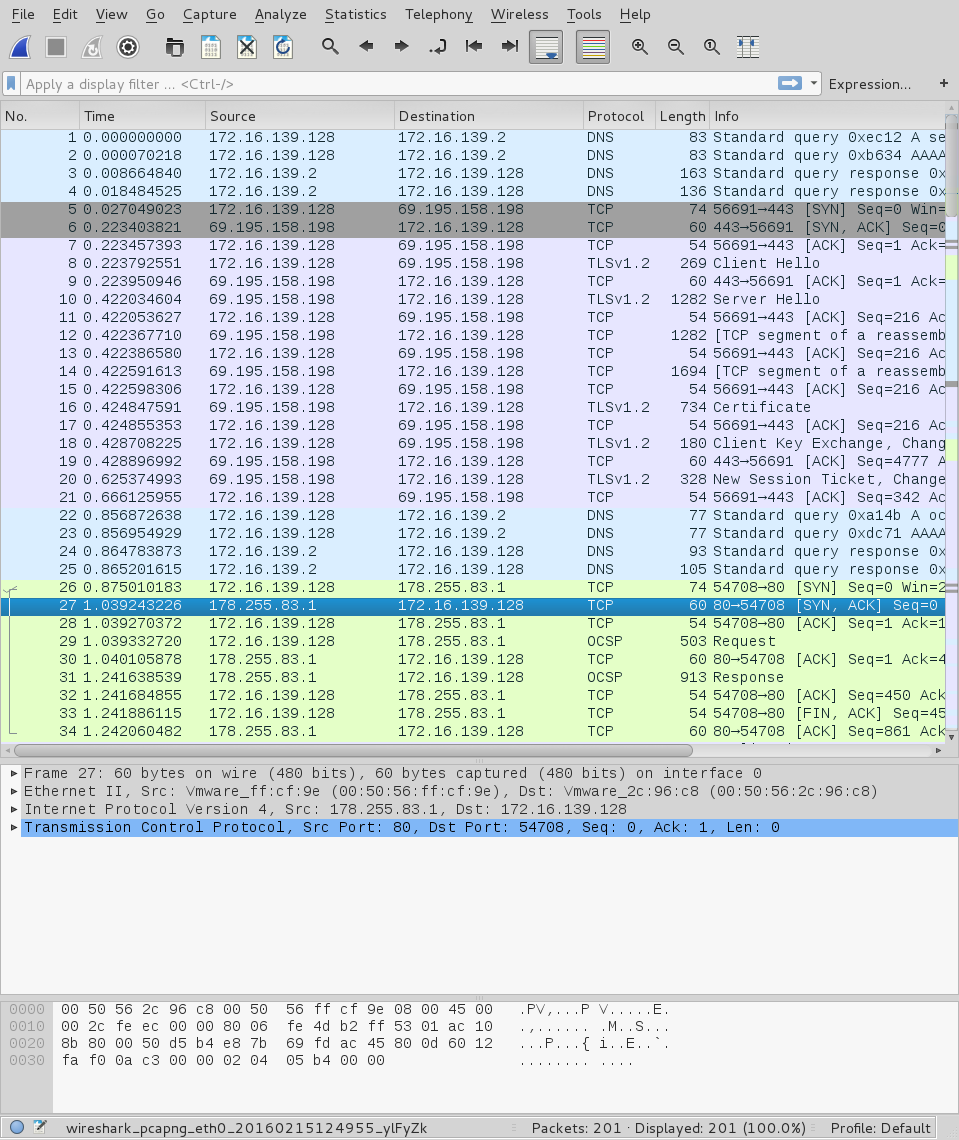
\includegraphics[scale=0.33]{./WiresharkAnalysis.png}
					\caption{Wireshark Capture Screen}
					\label{fig:WiresharkAnalysis}
			\end{figure}
			In this, there are four main areas to focus on:
			\begin{description}
				\item[Filter Toolbar] This toolbar is used to find the packet or type of packet that you are looking for. 
					It has it's own syntax which allows it to filter the packets which have been captured by items such as
					Protocol, type, source address or destination address. 
					This is one of the more powerful parts of Wireshark. 
				\item[Packet List] This is where you will spend much of your time. 
					The packet list is used to find the packet that you are searching for, and is found in the middle of the screen. 
					It is colour coded in a manner which can be found within the colour settings on the toolbar. 
					Between the detail found here, the colour coding and the filter toolbar, you should be able to find all packets that you require. 
				\item[Packet Details]
					This is directly below the packet list and contains the full metadata of the packet. 
					It is the location where you will find most of the interesting data which is encoded with the packets, but not a part of their data payload. 
				\item[Packet Bytes]
					This is a direct hexadecimal representation of the bytes which were sent as the packet. 
					It shows hex on one side and ASCII on the other, allowing for any plain text to be discovered. 
					Bytes which do not map to an ASCII code will be displayed as a full stop. 
			\end{description}
			
	\section{Netflow}
	\section{Malicious Website Analysis}
		After receiving a phishing email or another type of malicious link, it can be interesting and enlightening to look over how the exploit would have worked. 
		This process can be done in a relatively safe manner through the use of certain tools and sandboxes. 

		\subsection{Initial Analysis}
			When you first receive the email or link, you should analyse its content for external resources or identifying marks.
			This allows you to determine what parts of the link you should remove to ensure that your analysis cannot be traced back to you. 
			Furthermore, it allows you to determine if they have a method of tracking whether the email was opened, such as requesting an image from a remote source. 

			Once you have altered these tracing elements, you should be able to use the link provided to conduct an analysis. 
			However, at this point, under no circumstances should you enter the URL into your browser. 

		\subsection{Site Analysis}
		\index{Virus Total}
			You should first send the link through a scanner such as \href{virustotal.com}{Virus Total}. 
			This will tell you whether the site is loading anything commonly known to be malicious. 
			However, passing this does not mean the site is clean. 
			There may be content that has been created for this exploit which would not be picked up by the virus scanners the site runs. 

			The next step would be to use a site like \href{shrinktheweb.com}{Shrink the web} to view the site. 
			This allows you to view the content of the page without directly browsing to it, 
			saving you from risking your machine by accessing the page directly. 

			You may also want to look at domain registry records (whois records) to determine whether the site has recently been stolen or taken over. 
			This will give you detail on who owns the site and where it is located. 

			If neither of these actions work, it may be worthwhile continuing to the final phase. 

		\subsection{Direct Analysis}
			This should only be done if the previous actions did not lead to a useable solution. 
			Before conducting this, you should create an instance of a VM such as Kali that can be burnt after you have finished. 
			This process will likely infect the machine, so you should turn off all communication with the host system before beginning. 

			You should load a proxy such as burp suite, passing all traffic through this to check what is being sent. 
			It may also be worth loading Wireshark to allow you to track all packets sent during the session. 

			At this point, take the anonymised link and enter it into your browser. 
			This should begin the exploit, which you will be able to watch in both burp and Wireshark. 

			Check the traffic being sent for file downloads or javascript. 
			These will likely be the files that are run to start the malicious program. 
			From here, the process moves from analysis of a site to malware analysis, which will be covered in part in chapter \ref{ch:ReverseEngineering}.
